%% The following is a directive for TeXShop to indicate the main file
%%!TEX root = diss.tex

\chapter{A Description of 3D Reconstruction}
\label{ch:3DRecon_Desc}
In Chapter~\ref{ch:3DRecon_ProbSpace}, we introduce a taxonomy of 3D reconstruction which categorizes algorithms based on the problem space that they can reliably work under, \ie a mapping from problem space to algorithm space. However, without a formal description, \ie a model and representations, this mapping would be largely empirical. Expressing the conditions within which an algorithm works well without a formal definition of the problem space prevents formulating a well defined problem.

In this chapter, we attempt to provide a description of the 3D reconstruction problem which allows for a well defined specification of the conditions surrounding the problem. This description abstracts away from the functional specification of \textit{how} to estimate a reconstruction. We first propose a formal definition of the 3D reconstruction problem in Section~\ref{sec:3DRecon_Def}. Next, section~\ref{sec:3DRecon_Model} proposes a model to 3D reconstruction by selecting various key \textit{aspects} of the problem space that are crucial for describing the appearance of the object. Section~\ref{sec:3DRecon_Rep} outlines concrete representations of the proposed model. Section~\ref{sec:3DRecon_Exp} provides examples of expressing common 3D reconstruction problems using the proposed model and representations. These following four layers represent the description of our accessible 3D reconstruction framework: Definition, Representation, Model, and Expression.

% Computer vision problems require, among other factors, a model of the problem domain~\cite{little1985phdthesis} and appropriate representations. The model characterizes the relevant properties of the elements in the domain and analyze their relations. The representations describe an object's properties selected by the model to facilitate a solution of the problem.

\section{Model}
\label{sec:3DRecon_Model}
Models and representations are fundamental for vision problem solving. Models select characteristic properties of an object, and representation describes the model selected object properties to facilitate a solution of a class of problem. A model facilitates the representation of aspects in reality that are useful in a particular problem domain~\cite{bolles19863dpo}. For instance, surface orientation is one component of the surface geometry model, and the corresponding representation can be surface normal or curvature. Another example is colour, which is a component of a material model, and where RGB space is the corresponding representation of the colour.

We select the subset of properties used for object taxonomy in Chapter~\ref{ch:3DRecon_Taxo} as the main components of our model. The model consisting of these key properties is shown in Table~\ref{tab:3DRecon_model}.
\begin{table}[!htbp]
  \centering
  \begin{tabular}{l|l}
  \toprule
  \multirow{5}{*}{Model} & Texture\\
  & Lightness\\
  & Reflectance\\
  & Roughness\\
  & Concavity\\
  \bottomrule
  \end{tabular}
  \caption{Model of the 3D reconstruction problem. Properties are selected from the taxonomy in Chapter~\ref{ch:3DRecon_ProbSpace}.}
  \label{tab:3DRecon_model}
\end{table}

% In addition to these properties, there are requirements that can be imposed to the final reconstruction result. These requirements include but not exclude:

% \begin{table}[h]
%   \centering
%   \begin{tabular}{l|*{5}{c}}
%   \hline
%   \textbf{Requirement} & Accuracy-first & Completeness-first & Orientation-first & Roughness & Concavity\\
%   \hline
%   \end{tabular}
%   \caption{Model of the 3D reconstruction problem: requirements}
%   \label{tab:3DRecon_model}
% \end{table}

\section{Representation}
\label{sec:3DRecon_Rep}
Based on the proposed definition and model of the 3D reconstruction problem, we need to further define our representations so that the 3D reconstruction problem can be expressed using our proposed model. We need to turn our attention to how to represent the properties used in the proposed model.

% We look at the \textit{cues} that are utilized by 3D reconstruction techniques and their corresponding contributing properties. In Chapter~\ref{ch:3DRecon_Taxo}, we explored a new taxonomy of 3D reconstruction based visual/geometric cues. Now we need to investigate the visual and geometric properties of the object that can affect those cues. This section is organized by the visual/geomtric cues, and the visual/geomtric properties are investigated in each section.

% \subsection{Segment and scell}
% As defined in section~\ref{sec:3DRecon_Def}, a segment is the 3D to 2D transformation of a scell. Here we discuss concrete examples of segment and scell.

% \subsubsection{Pixel and voxel}
% In the image plane, a pixel is a square of size $1\times 1$. In the matrix representation of an image $I$, a pixel is an entry of the matrix, $I(x, y)$. A voxel is a 3D regular cube, and the center of which is projected to the center of the pixel.
% \begin{figure}[h]
% \centering
% 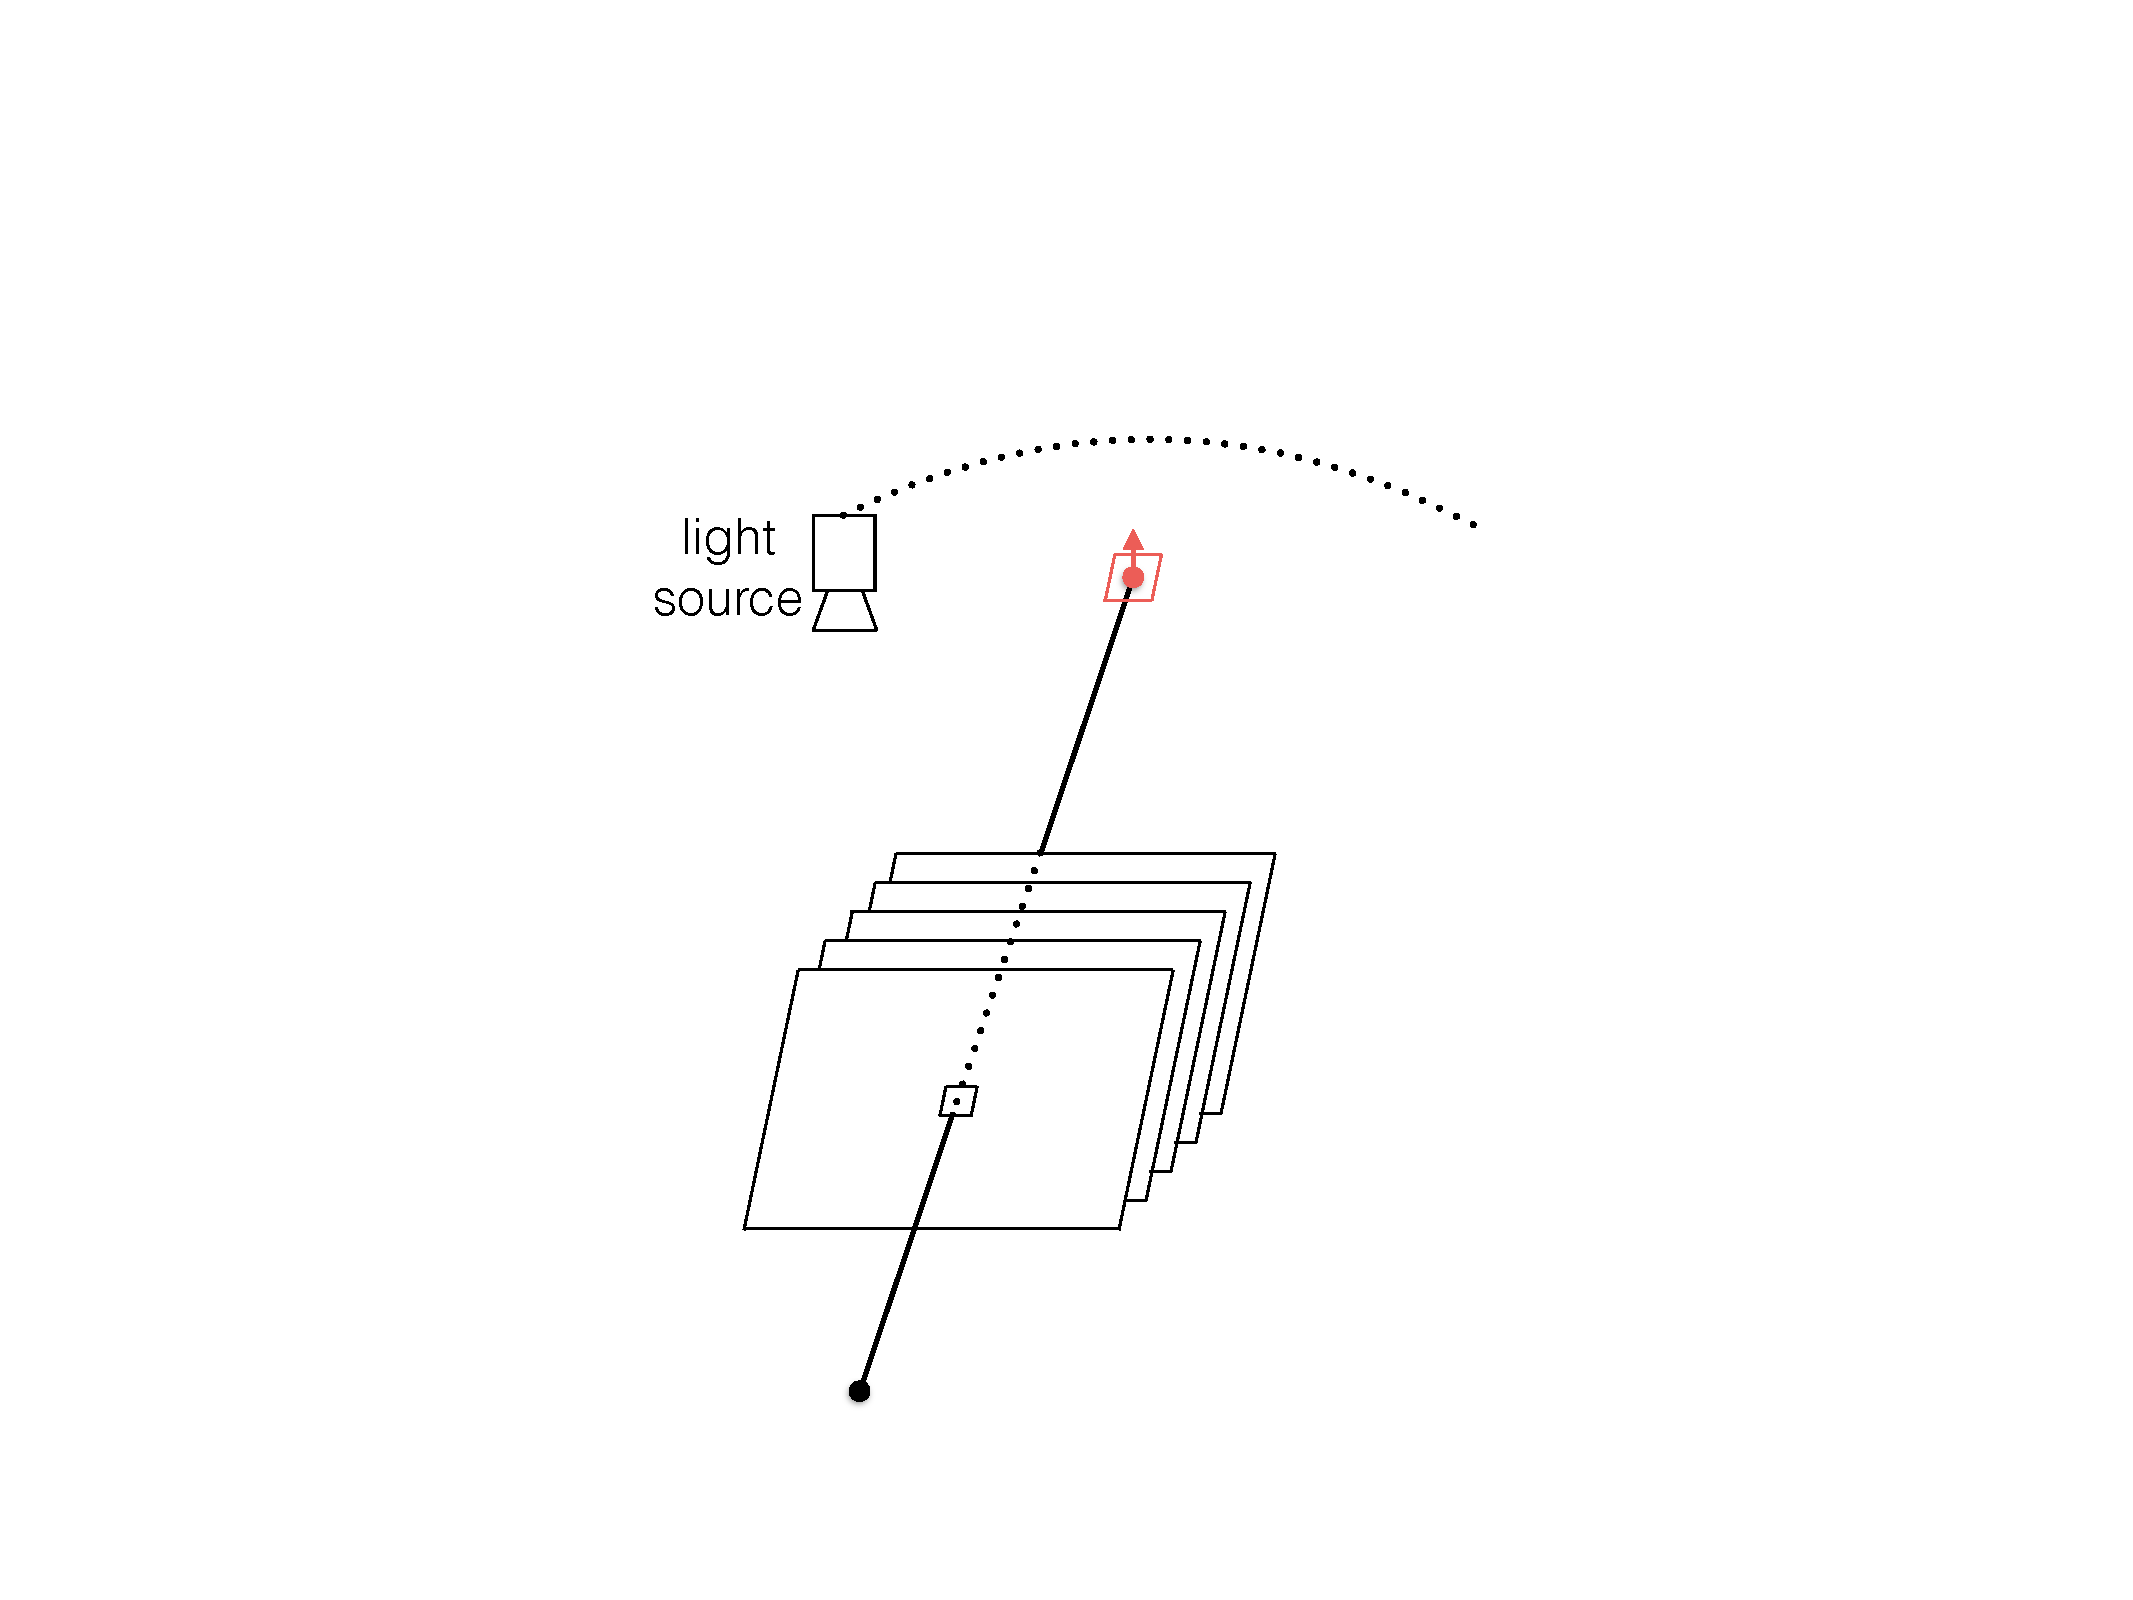
\includegraphics[width=0.5\texturewidth]{model/pixel_voxel}
% \caption{Pixel and voxel}
% \end{figure}

% \subsubsection{Silhouette and bounding edge}


% \subsubsection{Window area and patch}
% A window area is contained in a $w\times w$ regular square, and the surface patch is a 3D point of $p\times p$ with a normal vector.
% \begin{figure}[h]
% \centering
% 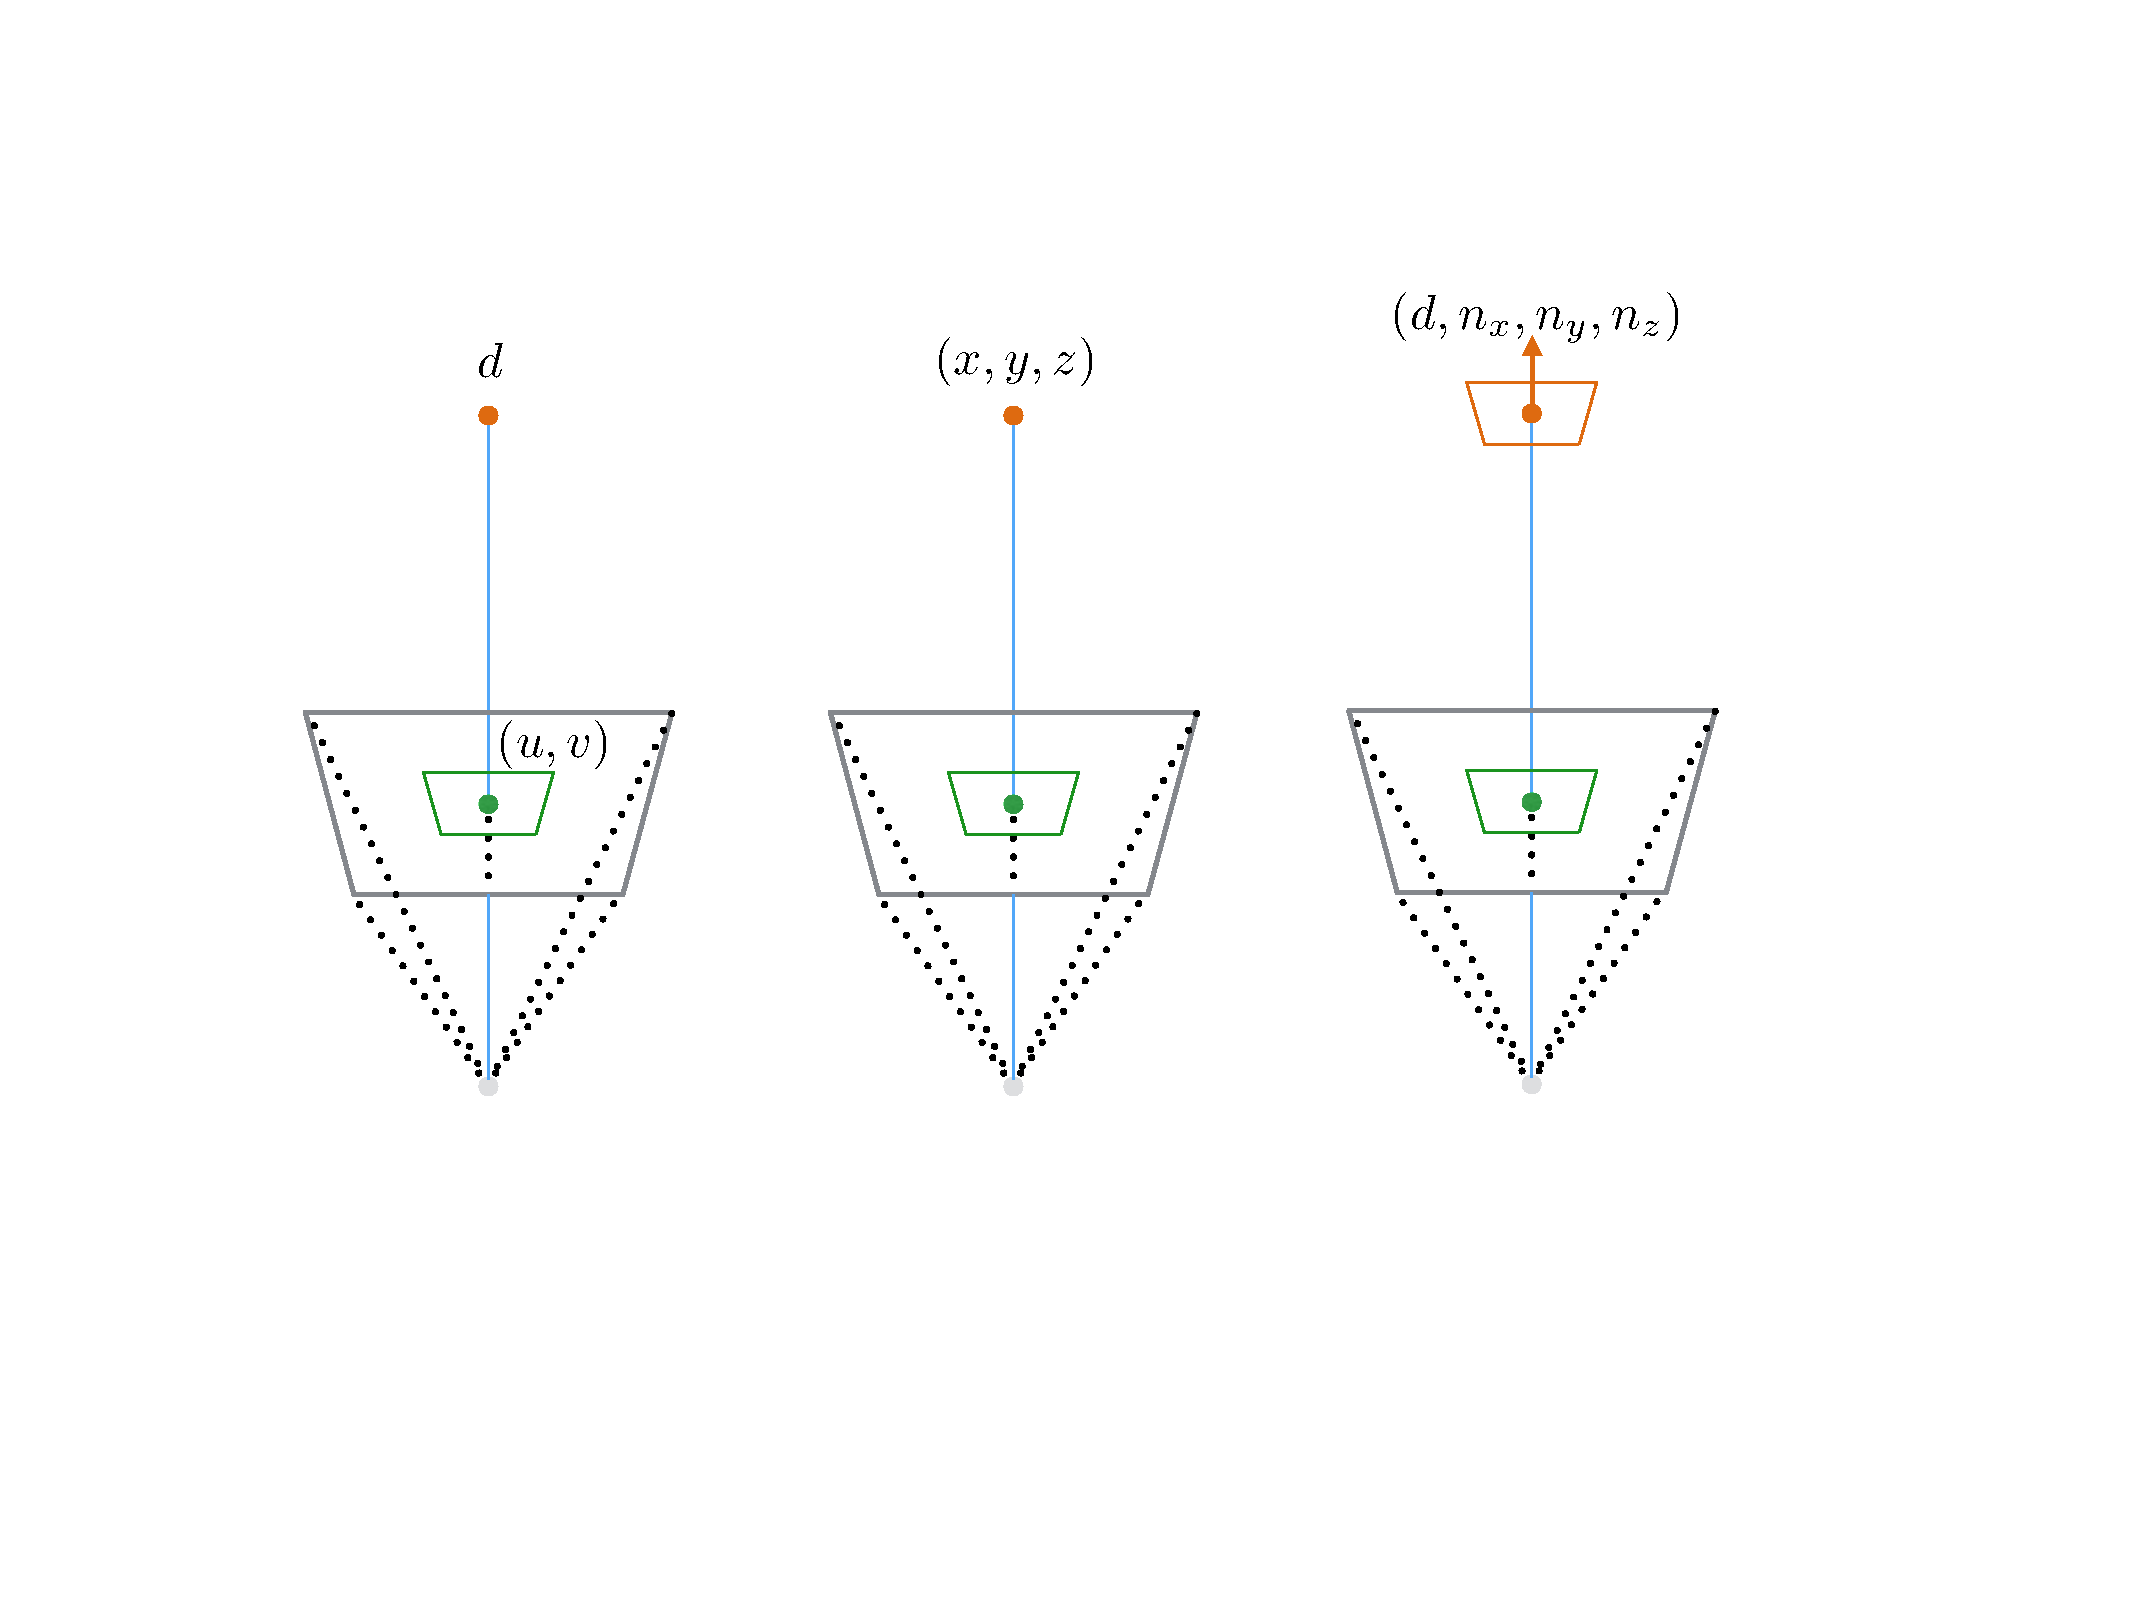
\includegraphics[width=0.8\textwidth]{model/window_patch}
% \caption{a window area and a surface patch}
% \end{figure}

% \subsection{Cues and properties}
% As defined in Chapter~\ref{sec:3DRecon_Def}, cue is the characteristics of the segment while property is that of the scell. For each cue observed in a segment, we discuss the underlying properties that have an impact on it.

\subsection{Texture}
Texture is one of the most important cues for many computer vision algorithms. It is generally divided into two categories, namely \textit{tactile} and \textit{visual} textures. Tactile textures refer to the immediate tangible feel of a surface, whereas visual textures refer to the visual impression that textures produce to the human observer, which are related to local spatial variations of simple stimuli like colour, orientation and intensity in an image. Here we focus only on visual textures, as they are more widely used in the stereo vision research. The term `texture' hereafter refers exclusively to `visual texture' unless mentioned otherwise.

Although texture is an important component in computer vision, there is no precise definition for the notion of texture itself. The main reason for this is that natural textures often exhibit separate yet contradicting properties, such as regularity versus randomness, or uniformity versus distortion, which can hardly be described in a unified manner. 
% Haralick considers a texture as an ``organized area phenomenon'' which can be decomposed into `primitives' having specific spatial distributions~\cite{haralick1979statistical}. This definition, also known as structural approach, comes directly from human visual experience of texture. These primitives are organized in a particular spatial structure indicating certain underlying placement rules. Alternatively, as Cross and Jain suggested, a texture is ``a stochastic, possibly periodic, two-dimensional image field''~\cite{cross1983markov}, which is also known as \textit{stochastic approach}.

% For s regular textures, there are two basic dimensions on which it may be described. The first dimension is for describing the primitives out of which the texture is composed, and the second dimension is for the description of the spatial dependence or interaction between the primitives of an image texture. The first property is concerned with tonal primitives and local properties, and the second dimension is concerned with the spatial organization of the tonal primitives.

There are various properties that make texture distinguishable: scale/size/granularity, orientation, homogeneity, randomness, etc. However, due to the diverse and complexe nature of textures, it is a challenging task to generate a synthetic texture solely from these semantic properties, or the other way around, derive parameters from a given texture. The stereo vision community often takes a simplified approach, classifying textures into two categories, regular and stochastic, by degree of randomness. A regular texture is formed by regular tiling of easily identifiable elements (texels) organized into strong periodic patterns. A stochastic texture exhibits less noticeable elements and displays rather random patterns. Most of the real world textures are mixtures of these two categories. In this thesis, we adopt this simplification and consider \textit{texture randomness}, which is the amount of distortion in the texture. Thus, a uniform texture has no/low \textit{texture randomness} whereas a highly textured surface has high \textit{texture randomness}.

% Most texture synthetic research has focused on data-driven or statistical approaches. For the data-driven approach, the generated texture is not general enough whereas it's not intuitive enough for the statistical approach. Thus we turn to an approach that is more tailored to the stereo vision problem. Based on the observations from practical tests, stereo algorithms work well under the condition of non-uniform texture, even for textures caused by shadow. This is theoretically plausible as stereo vision tries to find the correspondence based on the `distinctiveness' of the texture. Therefore, as long as the surface is covered by distinct texture, it doesn't matter what the basic texture element is. Thus the most significant attributes of the texture is coverage, \ie the percent of the surface that is covered, and it's the focus of this thesis.

% Texture is formally defined as a set of texture element or \textit{texels} occuring in some regular, or repeated, or random pattern. Texture gives us information about the \textit{spatial arrangement} of the colours or intensities in an image. However, it is something that is easy to recognize, but hard to define. 

% Here we only consider visual textures, which is the result of shape and reflection. Therefore, a surface with varying reflectance property can produces a textured surface, a flat surface with fixed reflectance property under different illuminations can also achieve textured effect. Even very weak texture can be a strong cue to object reconstruction as manifested by the Middlebury `Dino' dataset.

\subsection{Lightness}
When light strikes a surface, it may be reflected, transmitted, absorbed, or scattered; usually, a combination of these effects occurs. The intensity/colour information received by a sensor is thus determined, among other factors, by the amount of light available after these interactions. Here, we consider intensity as caused solely by reflection, since this is one of the most common phenomena experienced and is the easiest to analyze. Generally, we assume that all effects are local, thus global effects such as inter-reflection and transmission, among others, are omitted. This is called a \textbf{local interaction model}. 
% Lightness ranges from `black' to `white' in the grey scale axis, and colour is a superset of intensity, which takes into account the spectral composition of light. Both lightness and colour depend on illumination, surface normal, surface reflectance, and viewing direction.

In order to understand the contributing factors of pixel intensity/colour, we need an in-depth understanding of reflection, \ie how light is reflected off of a surface patch, and the relation between material and intensity values. The radiometric formation of an image consists of three separate processes, \textit{light-matter interaction}, \textit{light-lens interaction}, and \textit{light-sensor interaction}.

\subsubsection{Light-matter interaction}
The relation between the incoming illumination and reflected light is modelled using the \textit{bidirectional reflectance distribution function} (BRDF). The BRDF is defined as:

\noindent\textbf{Definition (BRDF)} the ratio of the scene radiance $\mathbf{L_r(\theta_r, \phi_r)}$ to the irradiance $\mathbf{E_i(\theta_i, \phi_i)}$, \ie $f(\theta_i, \phi_i, \theta_r, \phi_r)=\frac{E^{surface}(\theta_i, \phi_i)}{L^{surface}(\theta_r, \phi_r)}$.
\begin{figure}[!htbp]
\centering
\begin{tikzpicture}[node distance=2cm, auto]
\node (light_rad) [data] {Incident Radiance};
\node (material) [model, right of=light_rad, xshift=2cm] {Material};
\node (scene_rad) [data, right of=material, xshift=2cm] {Scene Radiance};
\draw [arrow] (light_rad) -- (material);
\draw [arrow] (material) -- (scene_rad);
\end{tikzpicture}
\caption{The light-matter interaction. Scene radiance is linear related to incident radiance.}
\label{fig:light_matter_interact}
\end{figure}

For Lambertian model, BRDF can be simplified as \textit{Diffuse albedo} or surface albedo, which is the proportion of incident light that is reflected by the surface. 
% It should be noted that albedo is not an intrinsic property of a surface. Instead, for any surface, the albedo depends on the spectral and angular distributions of the incident light.

\subsubsection{Light lens interaction}
A common assumption made in vision community is that radiance is constant as it propagates along a ray. Therefore, the scene radiance is the same as the radiance passing through the lens, which is the same as the radiance received by the sensor. Since image irradiance is the radiance accumulated on a unit surface, it follows that image irradiance is proportional to the scene radiance. Thus, the relation between \textit{scene radiance} and \textit{image irradiance} is linear.
\begin{figure}[!ht]
\centering
\begin{tikzpicture}[node distance=2cm, auto]
\node (scene_rad) [data] {Scene Radiance};
\node (lens) [model, right of=scene_rad, xshift=2cm] {Lens};
\node (irradiance) [data, right of=lens, xshift=2cm] {Image Irradiance};
\draw [arrow] (scene_rad) -- (lens);
\draw [arrow] (lens) -- (irradiance);
\end{tikzpicture}
\caption{The light-lens interaction. Image irradiance is linearly related to scene radiance.}
\label{fig:light_lens_interact}
\end{figure}

\subsubsection{Light sensor interaction}
The camera response function relating image irradiance at the image plane to measured pixel intensity values is a non-linear mapping. A linear relation can be retrieved by radiometric calibration.
\begin{figure}[!ht]
\centering
\begin{tikzpicture}[node distance=2cm, auto]
\node (irradiance) [data] {Image Irradiance};
\node (sensor) [model, right of=irradiance, xshift=2cm] {Sensor};
\node (intensity) [data, right of=sensor, xshift=2cm] {Intensity};
\draw [arrow] (irradiance) -- (sensor);
\draw [arrow] (sensor) -- (intensity);
\end{tikzpicture}
\caption{The light-sensor interaction. Pixel intensity is linearly related to image irradiance assuming linear radiometric mapping.}
\label{fig:light_sensor_interact}
\end{figure}

In conclusion, as long as the \textit{light-sensor interaction} is considered as a linear mapping (as most vision algorithms do) or calibrated in a pre-processing step, the pixel intensity value is linearly related to surface reflectance, which is characterized by BRDF. There are 4 DoF in spatially-invariant BRDF, and for the simplified case - Lambertian reflectance, the BRDF is degenerated to \textit{diffuse albedo}, which is the representation we adopt for lightness.

% The reflectance of light also depends on the incident direction. Specifically, light that lands on a surface at a grazing angle will be much more likely to reflect, see Figure~\ref{fig:alb_ang}. We take into account the Fresnel effect in the synthetic stage, thus we consider the albedo with small incident angle.
% \begin{figure}[h]
% \centering
% 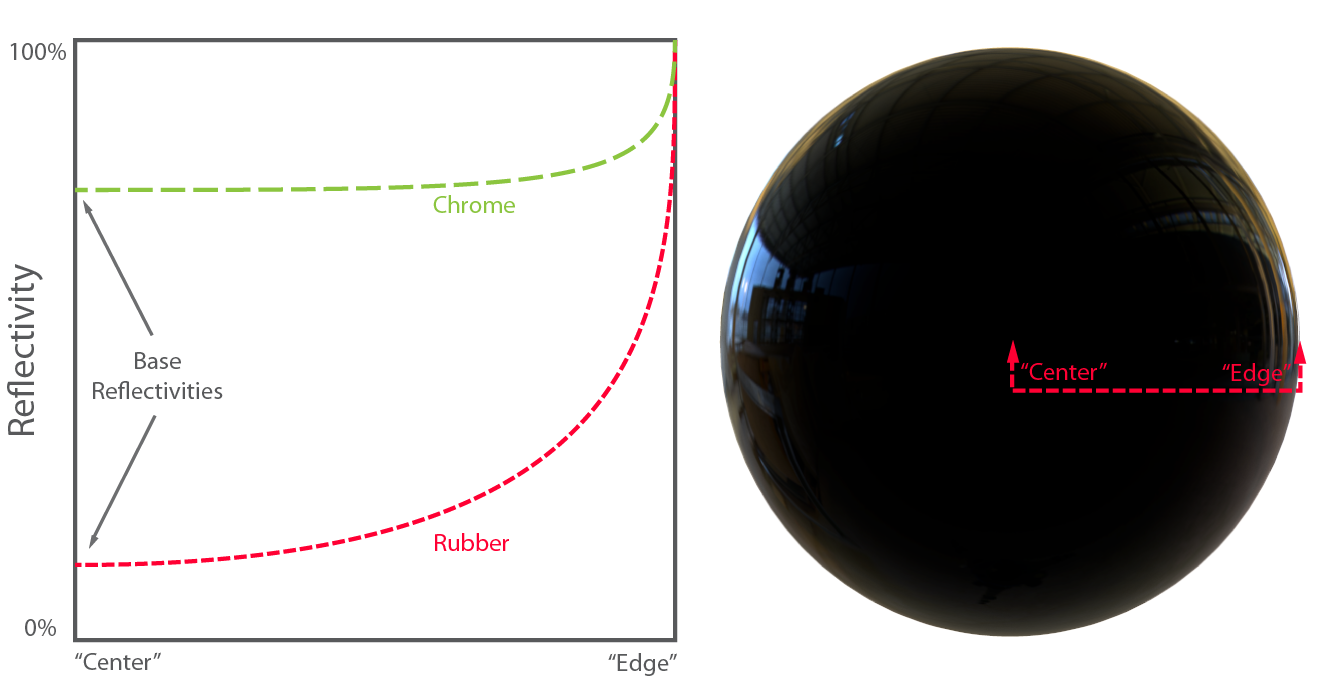
\includegraphics[width=0.5\textwidth]{model/reflectance_angle}
% \label{fig:alb_ang}
% % \caption{Spectral reflectance curves for aluminium (Al), silver (Ag), and gold (Au) metal mirrors at normal incidence.}
% \end{figure}

\subsection{Specularity}
Specular surfaces reflect light in nearly a single direction when microscopic surface irregularities are small compared to light wavelength, and no subsurface scattering is present~\cite{nayar1989surface}. Unlike diffuse reflections, where we experience the lightness and colour of an object, specular reflections carry information about the structure, intensity, and spectral content of the illumination field. In other words, specular reflection is simply an image of the environment, or the illumination field, distorted by the geometry of the reflecting surface. For instance, the specular sphere in Figure~\ref{fig:spec_ref} shows a distorted image of the environment instead of the underlying surface colour. A purely specular surface is a mirror, which is rare in nature. Most natural materials exhibit a mixture of specular and diffuse reflections. A commonly used model treats mixed reflectance as a weighted combination of diffuse and specular component. Thus the ratio of incident light that is specularly reflected is considered as the representation of sepcularity, with 0 being completely diffuse, and 1 being completely specular (mirror like).
%  We use a numeric \textit{specular} value to denote the proportion of a material's specularity.
\begin{figure}[!htbp]
\centering
\begin{tabular}{cc}
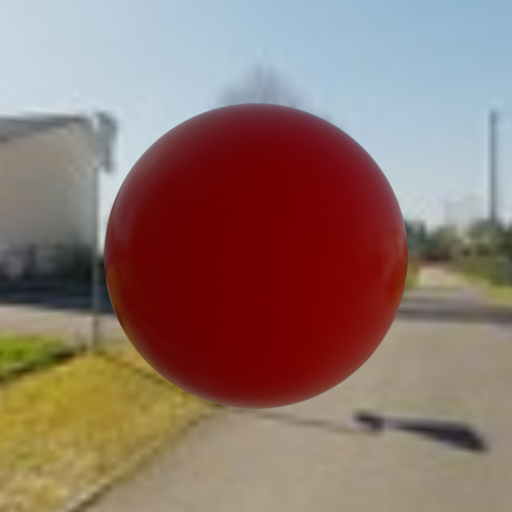
\includegraphics[width=0.3\textwidth]{model/sphere_diffuse}&
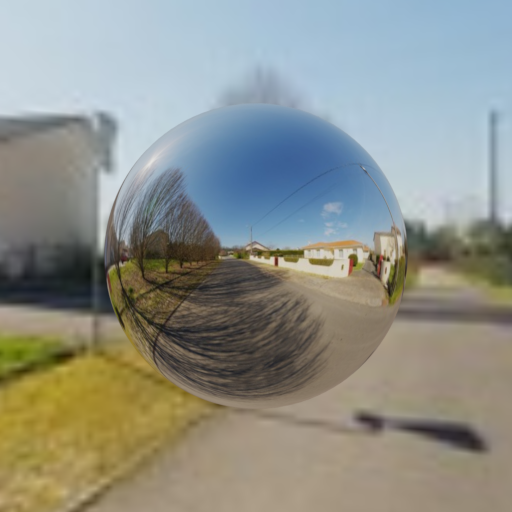
\includegraphics[width=0.3\textwidth]{model/sphere_specular}\\
(a) & (b)\\
\end{tabular}
\caption{(a). A \textbf{red} diffuse sphere; (b). a \textbf{red} specular sphere. The surface reflects light in a mirror-like way, showing a distorted environment. Since no diffuse reflection exists, the colour of the surface is no longer visible.}
\label{fig:spec_ref}
\end{figure}

\subsection{Roughness}
Roughness, which refers to the microscopic shape characteristics of a surface, contributes to the way in which light is reflected off of a surface. A smooth surface may reflect incident light in a single direction, while a rough surface may scatter the light in various directions. Thus, variations in microscopic surface geometry can cause specular reflections to be scattered, blurring the image of the environment in an amount proportional to surface roughness. We need prior knowledge of the microscopic surface irregularities, or a model of the surface itself, to determine the reflection of incident light.

Possible surface models are divided into 2 categories: surfaces with exact known profiles and surfaces with random irregularities. An exact profile may be determined by measuring the height at each point on the surface by means of a sensor such as the stylus profilometer. This method tends to be cumbersome and impractical, hence, it is more reasonable to model the surface as a random process, where it is described by a statistical distribution of either its height above a certain mean level, or its slope with respect to its mean (macroscopic) slope. We use the second statistical approach as the representation of roughness.

% \textit{Height Distribution Model} The height coordinate of the surface is expressed as random function of the coordinates $x$ and $y$.
% \begin{figure}[h]
% \centering
% \includegraphics[width=0.5\textwidth]{model/surface_representation_1}
% \caption{Surface height distribution model}
% \end{figure}

% The shape of the surface is determined by the probability distribution of $h$. For instance, let $h$ be normally distributed, with mean value $\bar{h}=0$ and standard deviation $\sigma_h$. Then, the distribution of $h$ is given by:
% $$
% p_h(h)=\frac{1}{\sqrt{2\pi}\sigma_h}e^{-\frac{h^2}{2\sigma_h^2}}
% $$

% The $\sigma_h$ is the root-mean-square of $h$ and represents the roughness of the surface. The surface is not uniquely described by the distribution of $h$, as it does not tell us anything about the distance between the hills and valleys of the surface.

% The surfaces below have the same height distribution function, i.e., the same mean value and standard deviation. However, they don't resemble each other in appearance.
% \begin{figure}[h]
% \centering
% \includegraphics[width=8cm]{model/same_mean_sd}
% \caption{Surface height distribution model}
% \end{figure}

% An autocorrelation coefficient $C(\tau)$ is introduced, that determines the correlation (or lack of independence) between the random values assumed by the height $h$ at two surface points $(x_1, y_1)$ and $(x_2, y_2)$, separated by a distance $\tau$. The autocorrelation coefficient can be:
% $$
% C(\tau)=e^{-\frac{\tau^2}{T^2}}
% $$

% where $T$ is the *correlation distance*. Therefore, the above surfaces have small and large correlation distances respectively.

% \subsubsection{Slope Distribution Model}
% We can think of a surface as a collection of planar micro-facets. A large set of micro-facets constitutes an infinitesimal surface patch that has a mean surface orientation $\vec{n}$. Each micro-facet has its own orientation, which may deviate from the mean surface orientation by an angle $\alpha$.
% \begin{figure}[h]
% \centering
% 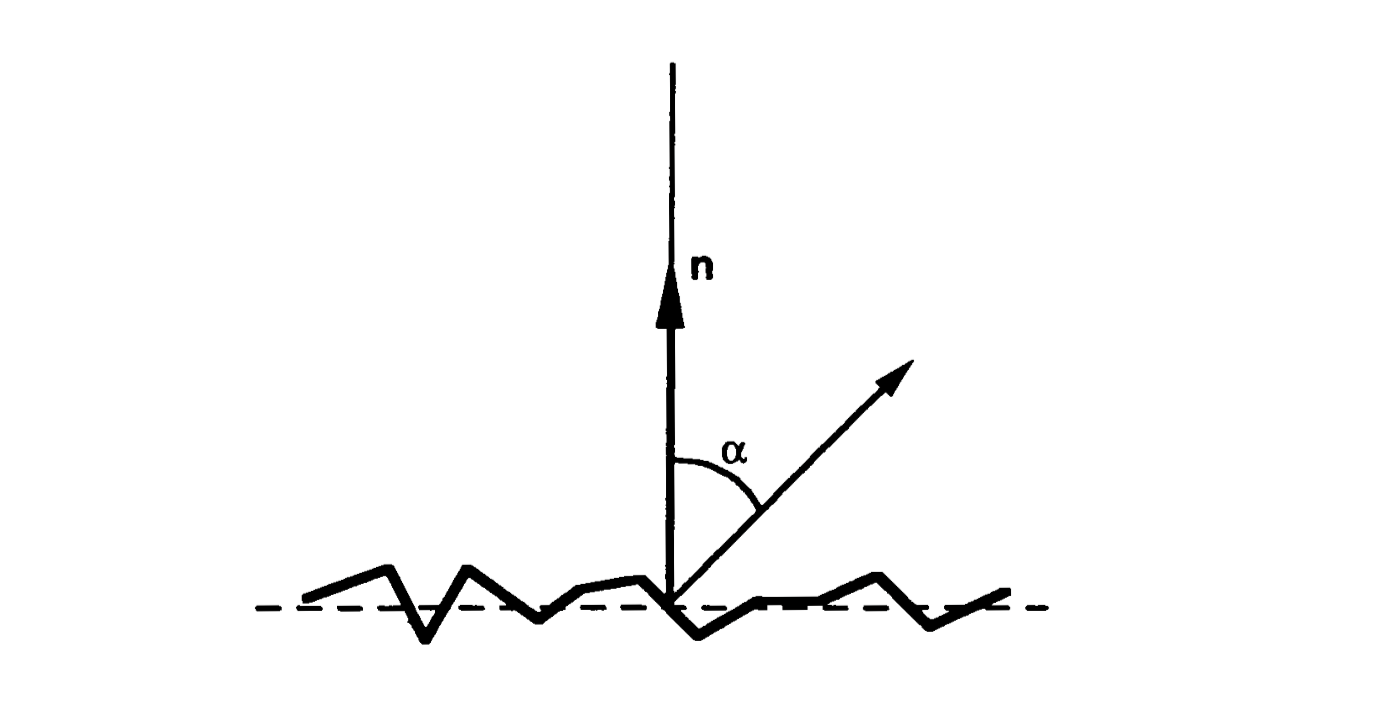
\includegraphics[width=0.7\textwidth]{model/surface_representation_2}
% \caption{Surface Slope Distribution Model}
% \end{figure}

% We will use the parameter $\alpha$ to represent the slope of individual facets. Surfaces can be modeled by a statistical distribution of the micro-facet slopes. If the surface is isotropic, the probability distribution of the micro-facet slopes can be assumed as rotationally symmetric w.r.t the mean surface normal $\vec{n}$.  Therefore, facet slopes can be described by a one-dimensional probability distribution function. For instance, the surface may be modeled by assuming a normal distribution for the facet slope $\alpha$, with mean value $\bar{\alpha}=0$ and standard deviation $\sigma_\alpha$, where the larger $\sigma_\alpha$ can be used to model rougher surfaces:
% $$
% p_\alpha(\alpha)=\frac{1}{\sqrt{2\pi}\sigma_\alpha}e^{-\frac{\alpha^2}{2\sigma_\alpha^2}}
% $$

% The surface model is determined by a single parameter $\sigma_\alpha$ While autocorrelation coefficient is important, the concept of slope correlation is more difficult to interpret and is not that useful in the generation of surface, which results in a weaker model compared to the height model. However, slope distribution model is popular in the analysis of surface reflection, as the scattering of light rays is dependent on the local slope of the surface and not the local height of the surface.

% surface roughness will affect the fresnel and specularity

% \subsection{Concavity}
% Concavity can be measured by \textit{surface curvature}, which is defined as the inverse of the radius of a tangentially intersecting circle/sphere. We include concavity in our model for the sake of completeness. However, we decide to omit this property in the following discussion since it will introduce global light transport including cast shadow and inter-reflection, and so on, which violates our assumption of \textbf{local interaction model}. Global light transport can severely worsen the accuracy of active methods. Besides, methods that utilize silhouette information may also fail to reconstruct concavities since concavity is invisible in the silhouette images.

\subsection{Perception of properties}
Human's visual system are extremly good at estimating material properties through vision. Being able to visually distinguish different material and infer their properties by vision is a critical capability for humans. For instance, when determining edibility, we can make subtle visual judgements of material properties to determine whether fruit is ripe, whether soup has bee left to go cold or whether bread is going stale~\cite{fleming2014visual}. There are numerous experimental evidence to support the intuition that human observers are good at recognizing and categorizing materials. For example, \citeauthor{sharan2009material} have shown that subjects can identify a wide range of materials from photographs even with brief presentations. \citeauthor{fleming2013perceptual} showed subjects photographs of materials from different categories and asked them to rate various subjective qualities, such as hardnesss, glossiness and prettiness. Even though subjects were not explicitly informed that the samples belonged to different classes, the subjective ratings of the individual samples were systematically clustered into categories, suggesting that subjects could theoretically classify materials through visual judgements of their properties.

Recently, \citeauthor{fleming2013perceptual} showed subjects photographs of materials from different categories and asked them to rate various subjective qualities, such as hardness, glossiness and prettiness. Even though subjects were not explicitly informed that the samples belonged to different classes, the subjective ratings of the individual samples were systematically clustered into categories, suggesting that subjects could theoretically classify materials through visual judgments of their properties.

There has been many efforts on the visual estimation of specific properties of materials, such as glossiness, translucency or surface roughness. For example, on the topic of glossiness, \citeauthor{nishida1998use} showed that subjects can judge the specular reflectance of computer simulated glossy surfaces.

On the topic of surface roughness, several authors have discussed how the visual system estimates and represents the characteristics of surface relief, although it remains unclear eaxctly which parameters of surface perturbations (e.g., scale, amplitude or profile) determine visual roughness, or indeed whether subjective roughness is a unitary quantity. Others have investigated how visual roughness relates to haptic impressions of roughness, although it is still not clear how the brain compares or integrates the two.

On the topic of perceived lightness, color. However, how the visual system distinguishes shading gradients that are caused by opaque reflectance from those that are caused by sub-surface scattering remains unclear, although shadow regions are likely to play a role, as these are the portions of objects that are most affected by light that has passed through the object.

In addition to visually inspection, we use the BRDF explorer developed by Disney Animation~\cite{disnybrdf} to visualize the rendered object with changing properties. A ``try-and-see'' approach was taken to obtain the parameters. More specifically, the user would change the value of each property and see if the rendered result resembles the real object. A similar approach can be found in~\cite{Berkiten:2016:ARB} where \citeauthor{Berkiten:2016:ARB} used a synthetic dataset to find the contributing factors of various Photometric Stereo algorithms.

The lightness of the object is controlled by the albedo value. Albedo is defiend as the ratio of reflected light with respect to incident light. The albedo is set as the value channel of HSV colour space. To determine the specularity and roughness of the object, we experiment with varying parameters to get the most realistic image. We demonstrate the process using the following example data `pot', as shown in Figure~\ref{fig:ui}.
\begin{figure}[!htbp]
\centering
\begin{tabular}{ccc}
  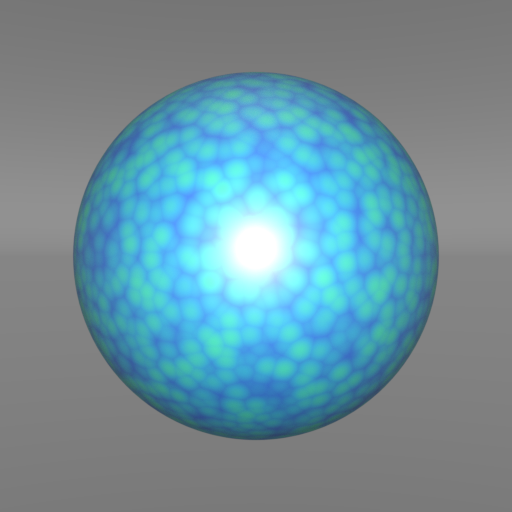
\includegraphics[width=0.3\textwidth]{interp/ui/ui_sphere.png}&
  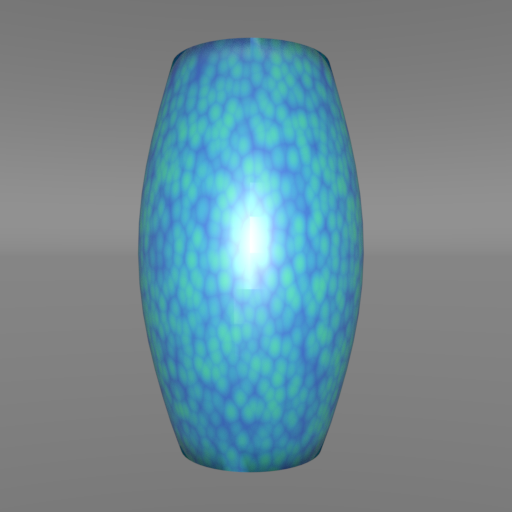
\includegraphics[width=0.3\textwidth]{interp/ui/ui_vase.png}&
  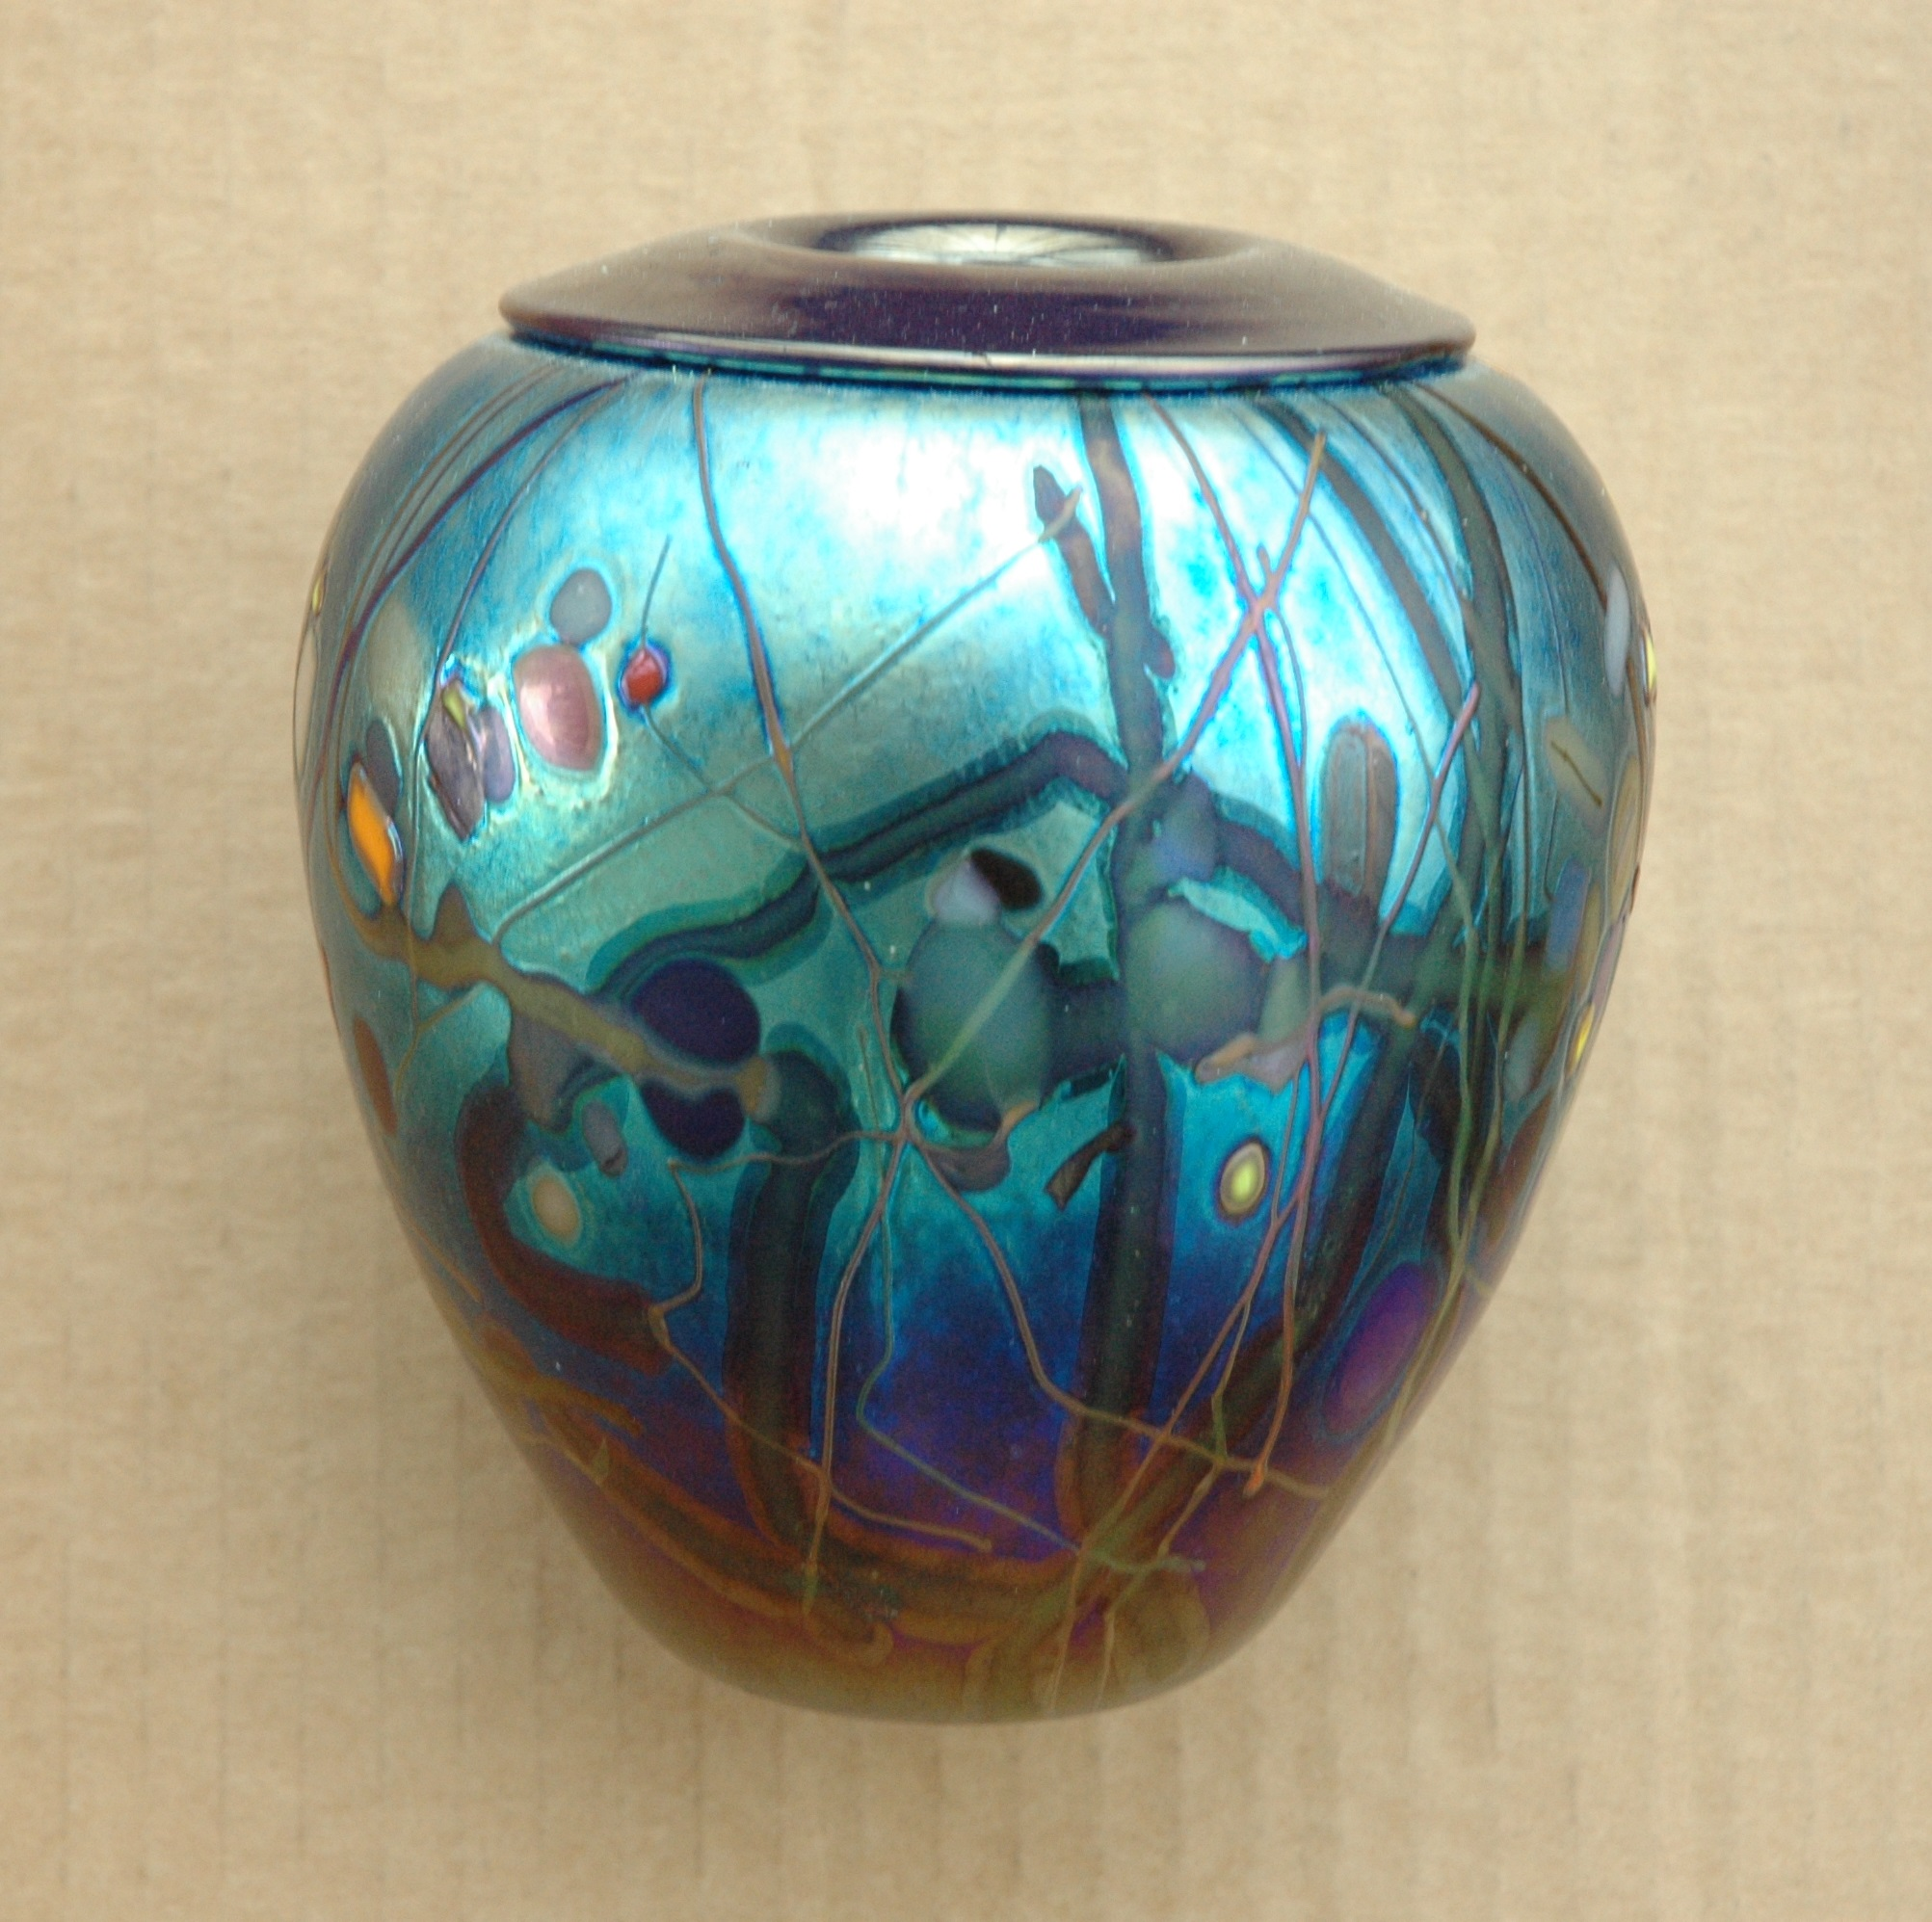
\includegraphics[width=0.3\textwidth]{img/interp/real_world_img/vase/vase.jpg}\\
  (a). synthetic sphere & (b). synthetic vase & (c). real-world vase\\
\end{tabular}
\caption{The UI for determining the property settings, including albedo, specular, and roughness of the surface. In this case shown above, the problem condition is: texture (0.8), albedo (0.8), specular (0.2), roughness(0.2). (a) demonstrates the effect of the property settings on a sphere, (b) on a teapot, and (c) shows the real-world object.}
\label{fig:ui}
\end{figure}

\subsection{Summary}
The model and corresponding rerpesentations are shown in Table~\ref{tab:3DRecon_model_repre}.
\begin{table}[!htbp]
  \centering
  \begin{tabular}{l|l}
  \toprule
  \textbf{Model} & \textbf{Representation}\\
  \midrule
  Texture & \textit{Texture randomness}\\
  Lightness & \textit{Diffuse albedo}\\
  Specularity & \textit{Specular reflectance}\\
  Roughness & \textit{SD of facet slopes}\\
  % Concavity & \textit{Surface curvature}\\
  \bottomrule
  \end{tabular}
  \caption{A Model and corresponding representations of the 3D reconstruction problem.}
  \label{tab:3DRecon_model_repre}
\end{table}

\section{Expression}
\label{sec:3DRecon_Exp}
Now that we have a proposed model and representations of 3D reconstruction problem, we can express the four proposed problem conditions using this description. Given that all perceived estimates would likely be low resolution from users, we use three discrete scales to parameterize these properties: \textit{low} (0.2), \textit{medium} (0.5), and \textit{high} (0.8). The expression of the reconstruction problem is shown in table~\ref{tab:express}.
\begin{table}[!htbp]
  \centering
  \begin{tabular}{l*{4}{p{1cm}}l}
  \toprule
  \textbf{Object} & Texture & Albedo & Specular & Rough & \textbf{Label}\\
  \midrule
  Class 1 & low/med & high & low/med & high & Tl-B-D-R\\
  Class 2 & low/med & high & high & low/med & Tl-B-M-S\\
  Class 3 & high & high & low/med & high & T-B-D-R\\
  Class 4 & high & high & high & low/med & T-B-M-S\\
  \bottomrule
  \end{tabular}
  \caption{Expression of the reconstruction problem for the four problem conditions proposed in Section~\ref{ch:3DRecon_ProbSpace}.}
  \label{tab:express}
\end{table}